\subsection{Exogenous IFIT1, IFIT3, and IFIT5 Localisation  During RSV Infection} \label{subsec:Exogenous IFIT1, IFIT3, and IFIT5 Localisation  During RSV Infection}
\subsubsection{OE IFIT1}
%hi1 + hrsv brsv
Detecting magenta: exogenous human IFIT1-FLAG \newline
Detecting cyan: h/bIB \newline
Cell Line: VERO \newline
Treatment: h/bRSV-GFP \newline

Overexpressed hIFIT1-FLAG colocalises with both human and bovine RSV IBs. This data is supported by evidence from z stacks.

\begin{figure}
    \centering
    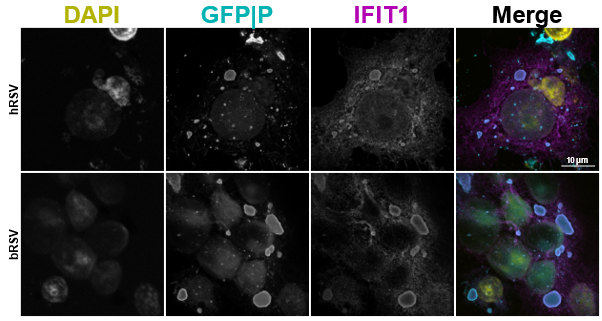
\includegraphics[width=1\linewidth]{09. Chapter 4/Figs/04. Overexpression/01. hi1 hrsv brsv.png}
    \caption[hi1 + hrsv brsv]{hi1 + hrsv brsv}
    \label{fig:hi1 + hrsv brsv}
\end{figure}

\subsubsection{OE IFIT3}
%bi3 + hrsv brsv
Cell Line: VERO \newline
Treatment: hRSV-GFP \newline
Detecting magenta: exogenous bovine IFIT3 \newline
Detecting cyan: human IB \newline

Overexpressed bIFIT3-FLAG was observed to colocalise with hRSV inclusion bodies (top panel; highlighted with arrows), as well as being excluded from the hRSV IBs, without any signs of IFIT3 signal on the periphery of the IB structures (middle and bottom panel). This data is supported by z stack measurements.

\begin{figure}
    \centering
    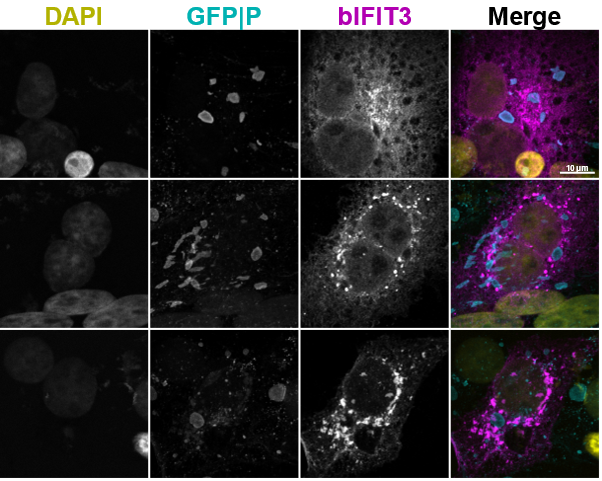
\includegraphics[width=1\linewidth]{09. Chapter 4/Figs/04. Overexpression/02. bi3 hrsv.png}
    \caption[bi3 + hrsv]{bi3 + hrsv}
    \label{fig:bi3 + hrsv}
\end{figure}

Cell Line: VERO \newline
Treatment: bRSV-GFP \newline
Detecting magenta: exogenous bovine IFIT3 \newline
Detecting cyan: bovine IB \newline

Very similar phenotype is observed for overexpressed bIFIT3-FLAG in bRSV infected cells. We see colocalization with IB (top panel) as well as exclusion from the structure without any signs of IFIT3 signal on the periphery of the IB structure (bottom panel). This data is as well supported by z stack measurements.

\begin{figure}
    \centering
    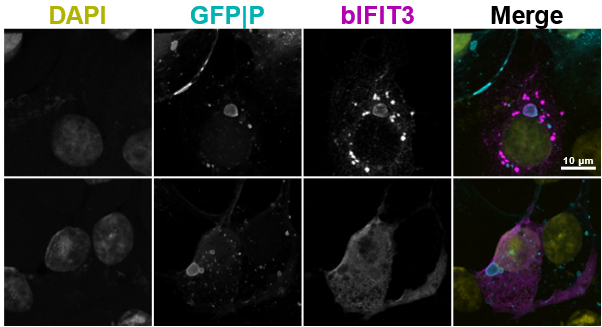
\includegraphics[width=1\linewidth]{09. Chapter 4/Figs/04. Overexpression/03. bi3 brsv.png}
    \caption[bi3 + brsv]{bi3 + brsv}
    \label{fig:bi3 + brsv}
\end{figure}


\subsubsection{OE IFIT5}
Detecting magenta: exogenous human IFIT5-FLAG \newline
Detecting cyan: h/bIB \newline
Cell Line: VERO \newline
Treatment: h/bRSV-GFP \newline

hIFIT5-FLAG is colocalising with hRSV inclusion bodies (basically resembling the P staining), while in bRSV infected cell there is a hint of IFIT5 signal concentration at the side of bRSV IB.

This data is by single cells per conditions as transfection did not work well. It is however supported by z stack measurements.


\begin{figure}
    \centering
    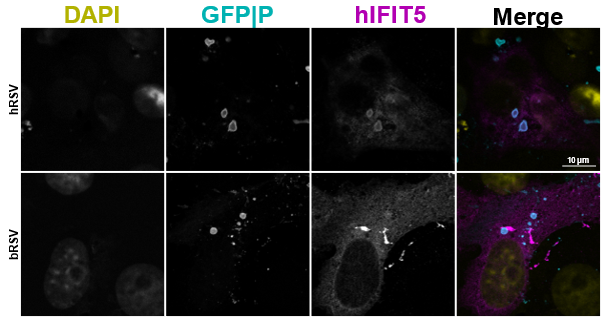
\includegraphics[width=1\linewidth]{09. Chapter 4/Figs/04. Overexpression/04. hi5-hrsv-brsv.png}
    \caption[hi5 + hrsv brsv]{hi5 + hrsv brsv}
    \label{fig:hi5 + hrsv brsv}
\end{figure}


\subsubsection{Summary} \label{Summary-oe}
Overexpressed hIFIT1-FLAG in the context of h/bRSV infection colocalises to both human and bovine IB structures.

Overexpressed bIFIT3 behaves equally between hRSV and bRSV infection, that is it sometimes colocalises with the IB structure and sometimes is completely excluded from the structure.

Overexpressed hIFIT5 in hRSV infected cells colocalises with the IBs.